\section*{Results}

In order to demonstrate that our method works, we run it on D-NeRF's synthetic
dataset which contains 8 different rendered scenes. These scenes have ground truth camera positions and viewing directions, as well as timestamps. They capture physically plausible movement, so there are no discontinuities or jumps between frames..

\subsection*{Quantitative Results}

The Bezier spline design is able to slightly outperform D-NeRF on their synthetic dataset. This is likely because D-NeRF can predict non-realistic movement, such as jumping from frame-to-frame, or suddenly accelerating. In practice, D-NeRF learns fairly smooth movement, but quantitatively looks different from our methods movement, which is likely due to variations in velocity and acceleration. Using Bezier spline, we enforce that movement is fluid, and thus can better reproduce missing frames. This leads to a small improvement in PSNR, because the dataset contains relatively simple movement, but we expect that in longer sequences or data with large gaps this difference would be more visible.

\subsection*{Qualitative Results}

The difference between our work and D-NeRF can be observed in the difference of flow between scenes. It's clear from Fig.~\ref{fig:dnerf_cmp} that our method more accurately captures squashing and stretching of movement, as the top of the ball is not moving but the bottom of the ball is falling. In contrast, D-NeRF contains approximately equal flow for the entire ball.

The difference between the two is also more clearly seen in videos of reconstruction. $C^0$-NeRF visibly has the effect of 'tweening between views, slowing into stops, while D-NeRF has more less smooth starts and stops. While it's difficult to characterize the plausibility of this movement, future work can measure smoothness of velocity and acceleration and use that as a way to differentiate between the approaches.

\begin{table*}[t]
    \centering
    \begin{tabular}{|c| c|c | c|c | c|c | c|c |}
    \hline
    \textbf{PSNR$^\uparrow$ $|$ MS-SSIM$^\uparrow$} & \multicolumn{2}{c|}{Bouncing Balls} & \multicolumn{2}{c|}{Hellwarrior} & \multicolumn{2}{c|}{Hook} & \multicolumn{2}{c|}{Jumping Jacks} \\
    \hline
    D-NeRF & \textbf{24.646} & \textbf{0.975}
           & 33.314 & 0.968
           & 27.954 & 0.978
           & 27.610 & \textbf{0.979} \\
    \hline
    $C^0$-NeRF & 24.251 & 0.971
               & \textbf{33.504} & 0.968
               & \textbf{28.104} & \textbf{0.979}
               & 27.610 & 0.978 \\
    \hline
    & \multicolumn{2}{c|}{Lego} & \multicolumn{2}{c|}{Mutant} & \multicolumn{2}{c|}{Standup} & \multicolumn{2}{c|}{T-Rex} \\
    \hline
    D-NeRF & \textbf{23.232} & \textbf{0.940}
           & 28.693 & 0.981
           & 31.218 & 0.989
           & \textbf{25.525} & \textbf{0.975} \\
    \hline
    $C^0$-NeRF & 23.148 & 0.938
               & \textbf{28.967} & \textbf{0.983}
               & \textbf{31.293} & 0.989
               & 25.421 & 0.972 \\
    \hline
    \end{tabular}
    \caption{
        Bezier splines are able to recover movement with slightly improved accuracy in dynamic scenes as compared to D-NeRF~\cite{pumarola2020dnerf}. Despite, or maybe because of, the forced prior of continuous movement, we are able to learn a smooth interpolation through each frame. We randomly samples all frames from the start of training, as opposed to D-NeRF which requires slowly introducing new frames, but we also remove the constraint that at time 0 D-NeRF must have no movement. Here, we parametrize $C^0$-NeRF with 6 control points.
    }
\end{table*}

\begin{figure*}
    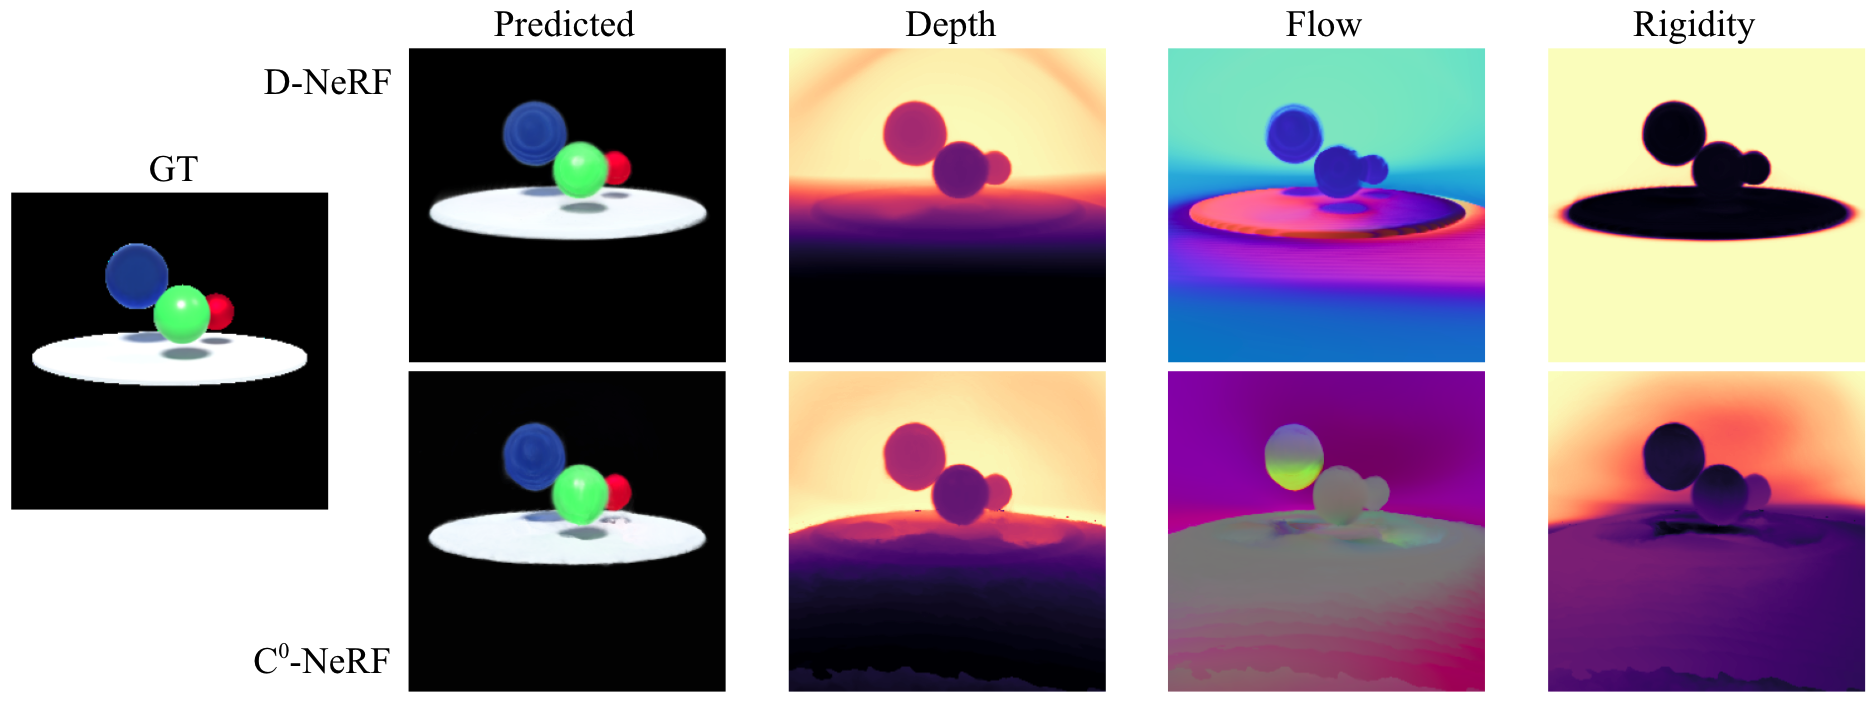
\includegraphics[width=\textwidth]{dnerf_compare}
    \caption{
        \label{fig:dnerf_cmp}
        Results comparing movement in D-NeRF~\cite{pumarola2020dnerf} versus Bezier-splines for a small timestep. There is substantial difference in the predicted flow, since D-NeRF cannot guarantee the initial frame has no movement. There is also a significant difference in rigidity, which is not easily explained. We believe it may be significantly easier to model low movement with splines, thus there is less of a need for rigidity.
    }
\end{figure*}
